\section{\autoref{chapter-routenplaner}, \nameref{chapter-routenplaner}}

\subsection*{\ref{subsection-aufgaben-routenplaner-modellierung} \nameref{subsection-aufgaben-routenplaner-modellierung}}

\begin{enumerate}
	\item Der Graph in \autoref{figure-graph-map-ch-solution} zeigt die Strassenkarte mit 17 Knoten.

\begin{figure}[htb]
\centering
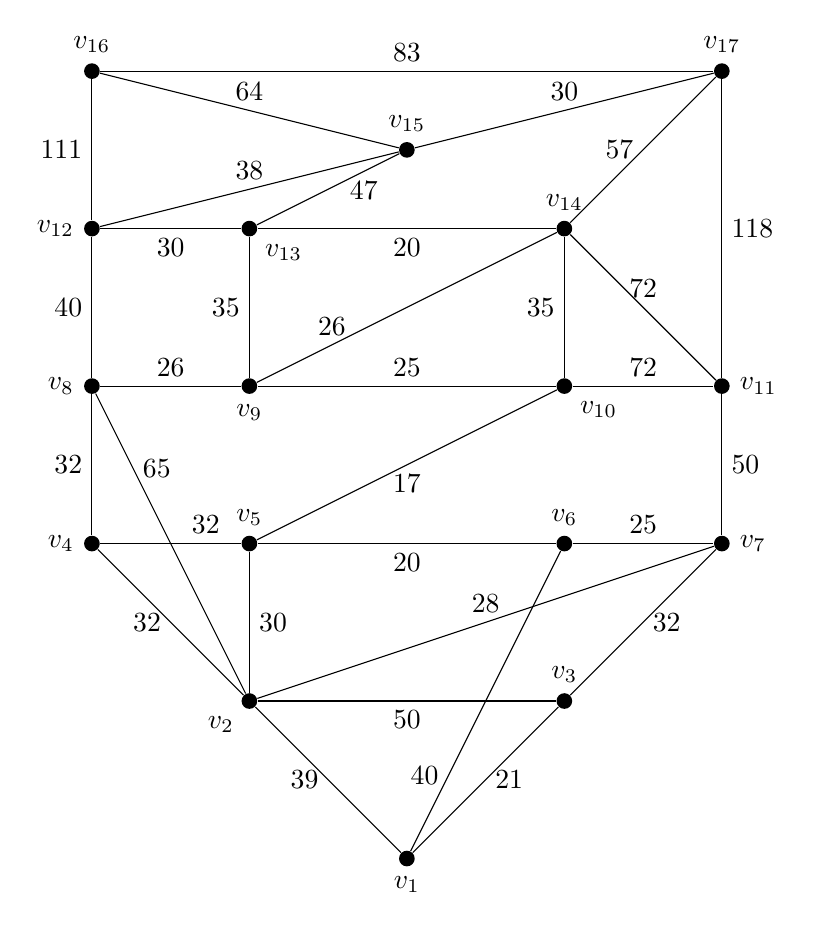
\begin{tikzpicture}
    \node[circle, fill, inner sep=2pt, label={south:$v_1$}] (v1) at (0,0) {};
    \node[circle, fill, inner sep=2pt, label={south west:$v_2$}] (v2) at (-2,2) {};
    \node[circle, fill, inner sep=2pt, label={$v_3$}] (v3) at (2,2) {};
    \node[circle, fill, inner sep=2pt, label={west:$v_4$}] (v4) at (-4,4) {};
    \node[circle, fill, inner sep=2pt, label={$v_5$}] (v5) at (-2,4) {};
    \node[circle, fill, inner sep=2pt, label={$v_6$}] (v6) at (2,4) {};
    \node[circle, fill, inner sep=2pt, label={east:$v_7$}] (v7) at (4,4) {};
    \node[circle, fill, inner sep=2pt, label={west:$v_8$}] (v8) at (-4,6) {};
    \node[circle, fill, inner sep=2pt, label={south:$v_9$}] (v9) at (-2,6) {};
    \node[circle, fill, inner sep=2pt, label={south east:$v_{10}$}] (v10) at (2,6) {};
    \node[circle, fill, inner sep=2pt, label={east:$v_{11}$}] (v11) at (4,6) {};
    \node[circle, fill, inner sep=2pt, label={west:$v_{12}$}] (v12) at (-4,8) {};
    \node[circle, fill, inner sep=2pt, label={south east:$v_{13}$}] (v13) at (-2,8) {};
    \node[circle, fill, inner sep=2pt, label={$v_{14}$}] (v14) at (2,8) {};
    \node[circle, fill, inner sep=2pt, label={$v_{15}$}] (v15) at (0,9) {};
    \node[circle, fill, inner sep=2pt, label={$v_{16}$}] (v16) at (-4,10) {};
    \node[circle, fill, inner sep=2pt, label={$v_{17}$}] (v17) at (4,10) {};
    \path (v1) edge node[left] {$39$} (v2);
    \path (v1) edge node[right] {$21$} (v3);
    \path (v1) edge node[left, near start] {$40$} (v6);
    \path (v2) edge node[below] {$50$} (v3);
    \path (v2) edge node[left] {$32$} (v4);
    \path (v2) edge node[right] {$30$} (v5);
    \path (v2) edge node[above] {$28$} (v7);
    \path (v2) edge node[right, near end] {$65$} (v8);
    \path (v3) edge node[right] {$32$} (v7);
    \path (v4) edge node[above, near end] {$32$} (v5);
    \path (v4) edge node[left] {$32$} (v8);
    \path (v5) edge node[below] {$20$} (v6);
    \path (v5) edge node[below] {$17$} (v10);
    \path (v6) edge node[above] {$25$} (v7);
    \path (v7) edge node[right] {$50$} (v11);
    \path (v8) edge node[above] {$26$} (v9);
    \path (v8) edge node[left] {$40$} (v12);
    \path (v9) edge node[above] {$25$} (v10);
    \path (v9) edge node[above, near start] {$26$} (v14);
    \path (v9) edge node[left] {$35$} (v13);
    \path (v10) edge node[left] {$35$} (v14);
    \path (v10) edge node[above] {$72$} (v11);
    \path (v11) edge node[above] {$72$} (v14);
    \path (v11) edge node[right] {$118$} (v17);
    \path (v12) edge node[below] {$30$} (v13);
    \path (v12) edge node[left] {$111$} (v16);
    \path (v12) edge node[above] {$38$} (v15);
    \path (v13) edge node[below, near end] {$47$} (v15);
    \path (v13) edge node[below] {$20$} (v14);
    \path (v14) edge node[left] {$57$} (v17);
    \path (v15) edge node[above] {$30$} (v17);
    \path (v15) edge node[above] {$64$} (v16);
    \path (v16) edge node[above] {$83$} (v17);
\end{tikzpicture}
\caption{Städte und Strassenkreuzungen werden zu Knoten.}
\label{figure-graph-map-ch-solution}
\end{figure}

\begin{multicols}{2}
\begin{itemize}
\item $v_1$ entspricht Olten
\item $v_2$ entspricht Solothurn
\item $v_3$ entspricht Dagmarsellen
\item $v_4$ entspricht Biel
\item $v_5$ entspricht einer Kreuzung
\item $v_6$ entspricht einer Kreuzung
\item $v_7$ entspricht einer Affoltern
\item $v_8$ entspricht Neuenburg
\item $v_9$ entspricht Kerzers
\item $v_{10}$ entspricht einer Kreuzung
\item $v_{11}$ entspricht Thun
\item $v_{12}$ entspricht Yverdon-les-Bains
\item $v_{13}$ entspricht einer Kreuzung
\item $v_{14}$ entspricht Freiburg
\item $v_{15}$ entspricht Lausanne
\item $v_{16}$ entspricht Genf
\item $v_{17}$ entspricht Montreux
\end{itemize}
\end{multicols}

\end{enumerate}

\subsection*{\ref{subsection-aufgaben-routenplaner-wege} \nameref{subsection-aufgaben-routenplaner-wege}}

\begin{enumerate}
	\item Der Weg ist in \autoref{figure-graph-11-solution} farblich hervorgehoben.
	
\begin{figure}[htb]
\centering
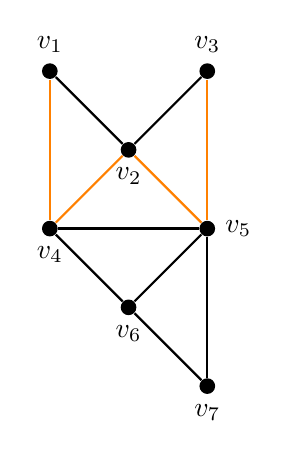
\begin{tikzpicture}
    \node[circle, fill, inner sep=2pt, label={north:$v_1$}] (v1) at (0,0) {};
    \node[circle, fill, inner sep=2pt, label={south:$v_2$}] (v2) at (1,-1) {};
    \node[circle, fill, inner sep=2pt, label={north:$v_3$}] (v3) at (2,0) {};
    \node[circle, fill, inner sep=2pt, label={south:$v_4$}] (v4) at (0,-2) {};
    \node[circle, fill, inner sep=2pt, label={east:$v_5$}] (v5) at (2,-2) {};
    \node[circle, fill, inner sep=2pt, label={south:$v_6$}] (v6) at (1,-3) {};
    \node[circle, fill, inner sep=2pt, label={south:$v_7$}] (v7) at (2,-4) {};
    \path (v1) edge[thick] (v2);
    \path (v1) edge[color=orange, thick] (v4);
    \path (v2) edge[thick] (v3);
    \path (v2) edge[color=orange, thick] (v4);
    \path (v2) edge[color=orange, thick] (v5);
    \path (v3) edge[color=orange, thick] (v5);
    \path (v4) edge[thick] (v5);
    \path (v4) edge[thick] (v6);
    \path (v5) edge[thick] (v6);
    \path (v5) edge[thick] (v7);
    \path (v6) edge[thick] (v7);
\end{tikzpicture}
\caption{Der Graph besitzt 7 Knoten und 11 Kanten.}
\label{figure-graph-11-solution}
\end{figure}

	\item Es gibt viele Wege. Ein Möglichkeit: $p = (v_1, v_4, v_5, v_6, v_7)$.
	\item Es gibt drei Wege: $p_1 = (v_1, v_2, v_3)$, $p_2 = (v_1, v_2, v_5, v_3)$, $p_3 = (v_1, v_4, v_5, v_3)$
	\item Es ist \textbf{kein} Weg, da zwischen $v_1$ und $v_3$ keine Kante existiert, die Knotenfolge in $p$ dies aber so verlangt.

\end{enumerate}

\subsection*{\ref{subsection-aufgaben-routenplaner-weglaenge} \nameref{subsection-aufgaben-routenplaner-weglaenge}}

\begin{enumerate}
	\item $l(p) = l((v_1, v_4, v_3)) = w(\{v_1, v_4\}) + w(\{v_4, v_3\}) = 8 + 12 = 20$
	\item $l(p) = l((v_1, v_2, v_3, v_4)) = w(\{v_1, v_2\}) + w(\{v_2, v_3\}) + w(\{v_3, v_4\}) = 2 + 42 + 12 = 56$
\end{enumerate}

\subsection*{\ref{subsection-aufgaben-routenplaner-brute-force} \nameref{subsection-aufgaben-routenplaner-brute-force}}

\begin{enumerate}
	\item Wir führen den Alle-Wege-Ausprobieren-Algorithmus aus \autoref{lst-algo-shortest-path-brute-force} Schritt-für-Schritt aus.	

\begin{itemize}
\item Input: Graph aus \autoref{figure-graph-14} mit Startknoten $s = v_4$ und Zielknoten $t = v_3$.
\item Schritt 1: Alle Wege von $s$ nach $t$ auflisten.

\begin{itemize}
	\item $p_1 = (v_4, v_2, v_3)$
	\item $p_2 = (v_4, v_5, v_3)$
	\item $p_3 = (v_4, v_1, v_2, v_3)$
	\item $p_4 = (v_4, v_2, v_5, v_3)$
	\item $p_5 = (v_4, v_5, v_2, v_3)$
	\item $p_6 = (v_4, v_1, v_2, v_5, v_3)$
\end{itemize}

\item Schritt 2: Für alle Wege aus dem 1. Schritt die Länge berechnen.

\begin{itemize}
\item $l(p_1) = 17$
\item $l(p_2) = 20$
\item $l(p_3) = 20$
\item $l(p_4) = 21$
\item $l(p_5) = 30$
\item $l(p_6) = 24$
\end{itemize}

\item Schritt 3: Weg mit minimaler Länge auswählen: $\underset{i}{\mathrm{arg~min}}~l(p_i) = 1$.

\item Output: $p_{1} = (v_4, v_2, v_3)$

\end{itemize}

	\item Wir führen den Alle-Wege-Ausprobieren-Algorithmus aus \autoref{lst-algo-shortest-path-brute-force} Schritt-für-Schritt aus.	
\begin{itemize}
\item Input: Graph aus \autoref{figure-graph-15} mit Startknoten $s = v_1$ und Zielknoten $t = v_9$.
\item Schritt 1: Alle Wege von $s$ nach $t$ auflisten.

\begin{itemize}
\item $p_1 = (v_1,v_3,v_5,v_2,v_4,v_7,v_9)$
\item $p_2 = (v_1,v_2,v_4,v_7,v_9)$
\item $p_3 = (v_1,v_2,v_5,v_7,v_9)$
\item $p_4 = (v_1,v_2,v_5,v_8,v_9)$
\item $p_5 = (v_1,v_2,v_4,v_7,v_5,v_8,v_9)$
\item $p_6 = (v_1,v_3,v_6,v_8,v_5,v_2,v_4,v_7,v_9)$
\item $p_7 = (v_1,v_3,v_5,v_7,v_9)$
\item $p_8 = (v_1,v_3,v_6,v_8,v_5,v_7,v_9)$
\item $p_9 = (v_1,v_2,v_5,v_3,v_6,v_8,v_9)$
\item $p_{10} = (v_1,v_2,v_4,v_7,v_5,v_3,v_6,v_8,v_9)$
\item $p_{11} = (v_1,v_3,v_6,v_8,v_9)$
\item $p_{12} = (v_1,v_3,v_5,v_8,v_9)$
\end{itemize}

\item Schritt 2: Für alle Wege aus dem 1. Schritt die Länge berechnen.

\begin{itemize}
\item $l(p_1) = 28$
\item $l(p_2) = 23$
\item $l(p_3) = 21$
\item $l(p_4) = 22$
\item $l(p_5) = 32$
\item $l(p_6) = 37$
\item $l(p_7) = 16$
\item $l(p_8) = 25$
\item $l(p_9) = 23$
\item $l(p_{10}) = 33$
\item $l(p_{11}) = 10$
\item $l(p_{12}) = 17$
\end{itemize}

\item Schritt 3: Weg mit minimaler Länge auswählen: $\underset{i}{\mathrm{arg~min}}~l(p_i) = 11$.

\item Output: $p_{11} = (v_1,v_3,v_6,v_8,v_9)$

\end{itemize}

\end{enumerate}

\subsection*{\ref{subsection-aufgaben-routenplaner-dijkstra} \nameref{subsection-aufgaben-routenplaner-dijkstra}}

\begin{enumerate}
	\item Wir führen den Dijkstra-Algorithmus für den Graphen aus \autoref{figure-dijkstra-aufgaben-g1} Schritt-für-Schritt aus und erhalten die Lösung aus \autoref{figure-dijkstra-aufgaben-g1-solution-1}.
	
\begin{figure}[htb]
\centering
\begin{minipage}{0.45\textwidth}
	\centering
	\begin{tikzpicture}
    \node[circle, fill, darkgreen, inner sep=2pt, label={[darkgreen]north:$v_1$}, label={[darkgreen]west:\textbf{0}}] (v1) at (0,0) {};
    \node[circle, fill, darkgreen, inner sep=2pt, label={[darkgreen]north:$v_2$}, label={[darkgreen]east:\textbf{2}}] (v2) at (4,0) {};
    \node[circle, fill, darkgreen, inner sep=2pt, label={[darkgreen]north east:$v_3$}, label={[darkgreen]east:\textbf{6}}] (v3) at (5,-2.5) {};
    \node[circle, fill, darkgreen, inner sep=2pt, label={[darkgreen]south:$v_4$}, label={[darkgreen]east:\textbf{8}}] (v4) at (4,-5) {};
    \node[circle, fill, darkgreen, inner sep=2pt, label={[darkgreen]south:$v_5$}, label={[darkgreen]west:\textbf{9}}] (v5) at (0,-5) {};
    \node[circle, fill, darkgreen, inner sep=2pt, label={[darkgreen]west:$v_6$}, label={[darkgreen]north east:\textbf{9}}] (v6) at (-1,-2.5) {};
    
    \node[circle, fill, darkgreen, inner sep=2pt, label={[darkgreen]north:$v_7$}, label={[darkgreen]east:\textbf{8}}] (v7) at (2,-1.5) {};
    \node[circle, fill, darkgreen, inner sep=2pt, label={[darkgreen]south east:$v_8$}, label={[darkgreen]north east:\textbf{12}}] (v8) at (1,-3.5) {};
    \node[circle, fill, darkgreen, inner sep=2pt, label={[darkgreen]south:$v_9$}, label={[darkgreen]north east:\textbf{9}}] (v9) at (3,-3.5) {};
    
    \path (v1) edge node[above] {$2$} node[darkgreen, below, thick] {$\leftarrow$}  (v2);
    \path (v2) edge node[right] {$4$} node[darkgreen, below, sloped, thick] {$\leftarrow$} (v3);
    \path (v3) edge node[right] {$2$} node[darkgreen, above, sloped, thick] {$\rightarrow$} (v4);
    \path (v4) edge node[below] {$1$} node[darkgreen, above, thick] {$\rightarrow$} (v5);
    \path (v5) edge node[left] {$6$} (v6);
    \path (v6) edge node[left] {$9$} node[darkgreen, below, thick, sloped] {$\rightarrow$} (v1);
    
    \path (v1) edge node[left] {$15$} (v7);
    \path (v2) edge node[below] {$6$} node[darkgreen, above, thick, sloped] {$\rightarrow$} (v7);
    \path (v3) edge node[below] {$15$} (v9);
    \path (v4) edge node[below] {$1$} node[darkgreen, above, thick, sloped] {$\rightarrow$} (v9);
    \path (v5) edge node[right] {$3$} node[darkgreen, above, thick, sloped] {$\leftarrow$} (v8);
    \path (v6) edge node[below] {$11$} (v8);
    
    \path (v8) edge node[below] {$4$} (v9);
    \path (v7) edge node[left] {$15$} (v8);
    \path (v7) edge node[right] {$2$} (v9);
    
    \begin{pgfonlayer}{background}
        \draw[rounded corners=2em, line width=2.25em, yellow!30, cap=round] (v1.center) -- (v2.center) -- (v3.center) -- (v4.center) -- (v9.center);
    \end{pgfonlayer}
\end{tikzpicture}
\caption{Der kürzeste Weg von $v_1$ zu $v_9$ lautet $p =(v_1, v_2, v_3, v_4, v_9)$.}
\label{figure-dijkstra-aufgaben-g1-solution-1}
\end{minipage}
\hfill
\begin{minipage}{0.45\textwidth}
	\centering
	\begin{tikzpicture}
    \node[circle, fill, darkgreen, inner sep=2pt, label={[darkgreen]north:$v_1$}, label={[darkgreen]west:\textbf{2}}] (v1) at (0,0) {};
    \node[circle, fill, darkgreen, inner sep=2pt, label={[darkgreen]north:$v_2$}, label={[darkgreen]east:\textbf{0}}] (v2) at (4,0) {};
    \node[circle, fill, darkgreen, inner sep=2pt, label={[darkgreen]north east:$v_3$}, label={[darkgreen]east:\textbf{4}}] (v3) at (5,-2.5) {};
    \node[circle, fill, darkgreen, inner sep=2pt, label={[darkgreen]south:$v_4$}, label={[darkgreen]east:\textbf{6}}] (v4) at (4,-5) {};
    \node[circle, fill, darkgreen, inner sep=2pt, label={[darkgreen]south:$v_5$}, label={[darkgreen]west:\textbf{7}}] (v5) at (0,-5) {};
    \node[circle, fill, darkgreen, inner sep=2pt, label={[darkgreen]west:$v_6$}, label={[darkgreen]north east:\textbf{11}}] (v6) at (-1,-2.5) {};
    
    \node[circle, fill, darkgreen, inner sep=2pt, label={[darkgreen]north:$v_7$}, label={[darkgreen]east:\textbf{6}}] (v7) at (2,-1.5) {};
    \node[circle, fill, darkgreen, inner sep=2pt, label={[darkgreen]south east:$v_8$}, label={[darkgreen]north east:\textbf{10}}] (v8) at (1,-3.5) {};
    \node[circle, fill, darkgreen, inner sep=2pt, label={[darkgreen]south:$v_9$}, label={[darkgreen]north east:\textbf{7}}] (v9) at (3,-3.5) {};
    
    \path (v1) edge node[above] {$2$} node[darkgreen, below, thick] {$\rightarrow$}  (v2);
    \path (v2) edge node[right] {$4$} node[darkgreen, below, thick, sloped] {$\leftarrow$} (v3);
    \path (v3) edge node[right] {$2$} node[darkgreen, above, thick, sloped] {$\rightarrow$} (v4);
    \path (v4) edge node[below] {$1$} node[darkgreen, above, thick] {$\rightarrow$} (v5);
    \path (v5) edge node[left] {$6$} (v6);
    \path (v6) edge node[left] {$9$} node[darkgreen, below, thick, sloped] {$\rightarrow$} (v1);
    
    \path (v1) edge node[left] {$15$} (v7);
    \path (v2) edge node[below] {$6$} node[darkgreen, above, thick, sloped] {$\rightarrow$} (v7);
    \path (v3) edge node[below] {$15$} (v9);
    \path (v4) edge node[below] {$1$} node[darkgreen, above, thick, sloped] {$\rightarrow$} (v9);
    \path (v5) edge node[right] {$3$} node[darkgreen, above, thick, sloped] {$\leftarrow$} (v8);
    \path (v6) edge node[below] {$11$} (v8);
    
    \path (v8) edge node[below] {$4$} (v9);
    \path (v7) edge node[left] {$15$} (v8);
    \path (v7) edge node[right] {$2$} (v9);
    
    \begin{pgfonlayer}{background}
        \draw[rounded corners=2em, line width=2.25em, yellow!30, cap=round] (v2.center) -- (v3.center) -- (v4.center) -- (v5.center);
    \end{pgfonlayer}
	\end{tikzpicture}
	\caption{Der kürzeste Weg von $v_2$ zu $v_5$ lautet $p = (v_2, v_3, v_4, v_5).$}
	\label{figure-dijkstra-aufgaben-g1-solution-2}
\end{minipage}
\end{figure}

	\item Der Algorithmus von Dijkstra liefert für einen Startknoten die kürzesten Wege zu allen anderen Knoten. Da der Startknoten gleich bleibt, können wir das Ergebnis aus der ersten Teilaufgabe wiederverwenden. Der kürzeste Weg lautet somit $p = (v_1, v_2, v_3,v _4)$.

	\item Da der Startknoten sich verändert hat, müssen wir den Dijkstra-Algorithmus erneut durchführen. Wir führen deshalb den Algorithmus für den Graphen aus \autoref{figure-dijkstra-aufgaben-g1} Schritt-für-Schritt aus und erhalten die Lösung aus \autoref{figure-dijkstra-aufgaben-g1-solution-2}.

\item Wir müssen den kürzesten Weg von $v_1$ nach $v_18$ bestimmen. Wir führen deshalb den Algorithmus für den Graphen aus \autoref{figure-dijkstra-aufgaben-g1} Schritt-für-Schritt aus und erhalten die Lösung aus \autoref{figure-dijkstra-aufgaben-g2-solution}.

\begin{figure}[htb]
\centering
\resizebox{!}{19cm}{
\begin{tikzpicture}
\begin{scope}[every node/.style={circle, thick, fill, darkgreen, draw, inner sep=0cm, minimum size=0.2cm}]
    \node[label={[label distance=0.1cm]180:$v_1$}, label={[darkgreen]north west:\textbf{0}}] (v1) at (-3,0) {};
    \node[label={[label distance=0.1cm]180:$v_2$}, label={[darkgreen]north:\textbf{8,2}}] (v2) at (-3,3) {};
    \node[label={[label distance=0.1cm]90:$v_3$}, label={[darkgreen]west:\textbf{9}}] (v3) at (0,6) {};
    \node[label={[label distance=0.1cm]270:$v_4$}, label={[darkgreen]north east:\textbf{11,3}}] (v4) at (2,3) {};
    \node[label={[label distance=0.3cm]90:\rotatebox{90}{$v_5$}}, label={[darkgreen]east:\textbf{7}}] (v5) at (6,0) {};
    \node[label={[label distance=0.1cm]90:\rotatebox{90}{$v_6$}}, label={[darkgreen]south west:\textbf{12,6}}] (v6) at (3,-3) {};
    \node[label={[label distance=0.1cm]180:$v_7$}, label={[darkgreen]north west:\textbf{10,5}}] (v7) at (-3,-3) {};
    \node[label={[label distance=0.1cm]90:$v_8$}, label={[darkgreen]south west:\textbf{15,7}}] (v8) at (3,6) {};
    \node[label={[label distance=0.2cm]0:$v_9$}, label={[darkgreen]north:\textbf{17,4}}] (v9) at (6,4) {};
    \node[label={[label distance=0.1cm]350:$v_{10}$}, label={[darkgreen]north east:\textbf{20}}] (v10) at (9,2) {};
    \node[label={[label distance=0.1cm]0:$v_{11}$}, label={[darkgreen]west:\textbf{13,2}}] (v11) at (7.5,-2) {};
    \node[label={[label distance=0.1cm]0:$v_{12}$}, label={[darkgreen]north west:\textbf{21}}] (v12) at (9,0) {};
    \node[label={[label distance=0.1cm]180:$v_{13}$}, label={[darkgreen]east:\textbf{23,2}}] (v13) at (12,-4) {};
    \node[label={[label distance=0.1cm]270:$v_{14}$}, label={[darkgreen]east:\textbf{17,7}}] (v14) at (7.5,-5) {};
    \node[label={[label distance=0.1cm]270:\rotatebox{90}{$v_{15}$}}, label={[darkgreen]east:\textbf{21,8}}] (v15) at (12,-8) {};
    \node[label={[label distance=0.5cm]270:\rotatebox{90}{$v_{16}$}}, label={[darkgreen]south east:\textbf{15,6}}] (v16) at (3,-8) {};
    \node[label={[label distance=0.1cm]180:$v_{17}$}, label={[darkgreen]north east:\textbf{21,7}}] (v17) at (-3,-8) {};
    \node[label={[label distance=0.1cm]180:$v_{18}$}, label={[darkgreen]north east:\textbf{24,6}}] (v18) at (0,-12) {};
    \node[label={[label distance=0.1cm]0:$v_{19}$}, label={[darkgreen]north:\textbf{30,1}}] (v19) at (5,-12) {};
\end{scope}
\begin{scope}[every edge/.style={draw=black, thick}]
    \path (v1) edge node[left] {$8,2$} node[darkgreen, below, near end, sloped] {$\leftarrow$} (v2);
    \path (v1) edge node[near end, right] {$9,0$} node[darkgreen, above, sloped, near end] {$\leftarrow$} (v3);
    \path (v1) edge node[above] {$7,0$} node[darkgreen, below, near end] {$\leftarrow$} (v5);
    \path (v1) edge node[right] {$10,5$} node[darkgreen, above, sloped, near end] {$\leftarrow$} (v7);
    
    \path (v3) edge node[right] {$2,3$} node[darkgreen, below, sloped, near end] {$\leftarrow$} (v4);
    \path (v3) edge node[above] {$6,7$} node[darkgreen, above, near end] {$\leftarrow$} (v8);
    
    \path (v4) edge node[near start, above] {$6,4$} node[darkgreen, below, sloped, near end] {$\leftarrow$} (v9);
    
    \path (v5) edge node[left] {$5,6$} node[darkgreen, below, near start, sloped] {$\leftarrow$} (v6);
    \path (v5) edge node[near end, above] {$13,0$} node[darkgreen, below, near end, sloped] {$\leftarrow$} (v10);
    \path (v5) edge node[near start, right] {$6,2$} node[darkgreen, below, near end, sloped] {$\leftarrow$} (v11);
    
    \path (v7) edge node[right] {$5,1$} node[darkgreen, below, sloped, near end] {$\leftarrow$} (v16);
    \path (v11) edge node[left] {$4,5$} node[darkgreen, above, sloped, near end] {$\leftarrow$}  (v14);
    \path (v12) edge node[right] {$7,8$} node[darkgreen, below, sloped, near start] {$\leftarrow$} (v11);
    \path (v14) edge[bend left=45, above] node {$5,5$} node[darkgreen, below, sloped, near end] {$\leftarrow$} (v13);
    \path (v15) edge node[below] {$6,2$} node[darkgreen, above, near start] {$\leftarrow$} (v16);
    \path (v16) edge node[below] {$6,1$} node[darkgreen, above, near end] {$\rightarrow$} (v17);
    \path (v17) edge node[left] {$2,9$} node[darkgreen, above, sloped, near end] {$\leftarrow$} (v18);
    \path (v18) edge node[above] {$5,3$} node[darkgreen, below, near end] {$\leftarrow$} (v19);
    
    \path (v1) edge node[above] {$13,4$} (v6);
    \path (v2) edge node[left] {$5,6$} (v3);
    \path (v2) edge node[above] {$4,6$} (v4);
    \path (v4) edge node[left] {$4,9$} (v5);
    \path (v5) edge node[left] {$14,3$} (v8);
    \path (v6) edge node[above] {$7,1$} (v7);
    \path (v6) edge node[above] {$5,9$} (v14);
    \path (v6) edge node[left] {$6,0$} (v16);
    \path (v7) edge node[left] {$11,6$} (v17);
    \path (v7) edge node[right, near start] {$18,2$} (v18);
    \path (v8) edge node[above] {$3,8$} (v9);
    \path (v8) edge[bend left=70, below] node {$6,6$} (v10);
    \path (v9) edge node[above] {$4,1$} (v10);
    \path (v9) edge[bend left=10] node[near start, left] {$5,8$} (v11);
    \path (v10) edge node[right] {$18,9$} (v12);
    \path (v12) edge node[left] {$11,8$} (v13);
    \path (v12) edge node[below] {$21,1$} (v6);
    \path (v13) edge node[left] {$12,1$} (v15);
    \path (v13) edge[bend left=20, below] node {$11,5$} (v16);
    \path (v14) edge node[right, near start] {$3,6$} (v16);
    \path (v15) edge[bend left=45, above] node {$15,6$} (v17);
    \path (v15) edge node[above] {$19,5$} (v18);
\end{scope}
\end{tikzpicture}
}
\caption{Der kürzeste Weg von $v_1$ zu $v_{18}$ lautet $p = (v_1, v_7, v_{16}, v_{17}, v_{18})$.}
\label{figure-dijkstra-aufgaben-g2-solution}
\end{figure}


\end{enumerate}